\documentclass[border=10pt,tikz]{standalone}
\usepackage[utf8]{inputenc}
\usepackage{tikz}
\usetikzlibrary{arrows.meta, positioning}
\usepackage{xcolor}

\definecolor{cRed}{HTML}{C0392B}
\definecolor{cPurple}{HTML}{8E44AD}
\definecolor{cGray}{HTML}{7F8C8D}

\begin{document}
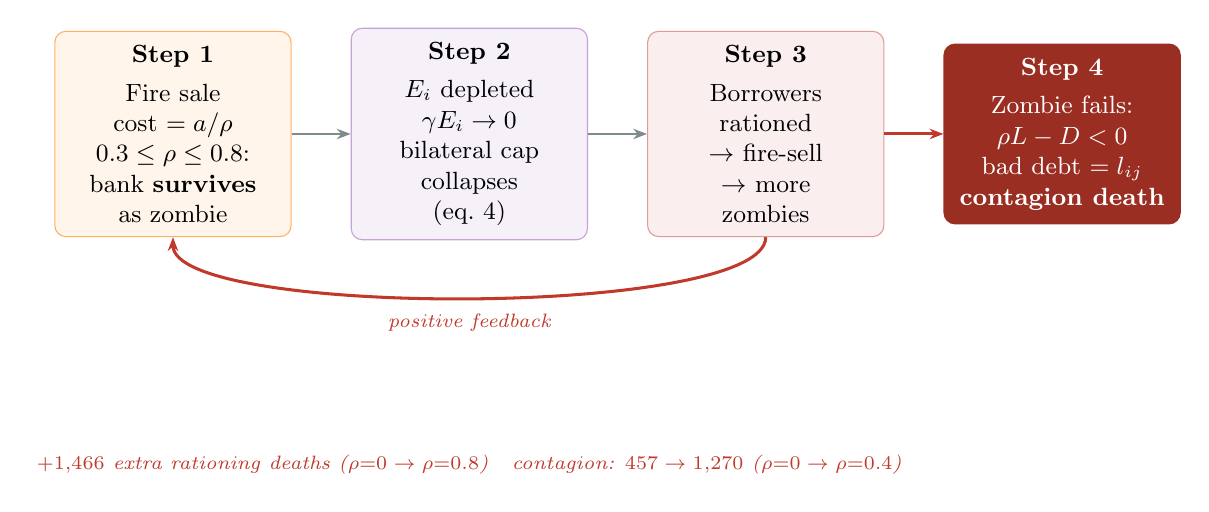
\begin{tikzpicture}[
  node distance=0.5cm and 0.75cm,
  zstep/.style={rectangle, rounded corners=4pt, draw, minimum width=3.0cm,
               minimum height=2.2cm, align=center, font=\small, inner sep=5pt},
  s1/.style={zstep, fill=orange!8, draw=orange!60},
  s2/.style={zstep, fill=cPurple!8, draw=cPurple!50},
  s3/.style={zstep, fill=cRed!8, draw=cRed!50},
  s4/.style={zstep, fill=cRed!80!black, draw=cRed!80!black, text=white},
  arr/.style={-{Stealth[length=5pt]}, line width=1pt, color=cGray},
  redarr/.style={-{Stealth[length=5pt]}, line width=1.1pt, color=cRed},
]
\node[s1] (s1) {\textbf{Step 1}\\[3pt]Fire sale\\cost $= a/\rho$\\$0.3\leq\rho\leq 0.8$:\\bank \textbf{survives}\\as zombie};
\node[s2, right=of s1] (s2) {\textbf{Step 2}\\[3pt]$E_i$ depleted\\$\gamma E_i\to 0$\\bilateral cap\\collapses\\(eq.~4)};
\node[s3, right=of s2] (s3) {\textbf{Step 3}\\[3pt]Borrowers\\rationed\\$\to$ fire-sell\\$\to$ more\\zombies};
\node[s4, right=of s3] (s4) {\textbf{Step 4}\\[3pt]Zombie fails:\\$\rho L-D<0$\\bad debt $=l_{ij}$\\\textbf{contagion death}};
\draw[arr]    (s1)--(s2);
\draw[arr]    (s2)--(s3);
\draw[redarr] (s3)--(s4);
\draw[redarr, out=-90, in=-90, looseness=0.35] (s3.south) to
  node[below, font=\scriptsize\itshape, color=cRed, yshift=-2pt]{positive feedback} (s1.south);
\node[font=\scriptsize\itshape,color=cRed,
      below=2.6cm of s2, anchor=north, align=center]
  {$+1{,}466$ extra rationing deaths ($\rho{=}0\to\rho{=}0.8$)\quad
   contagion: $457\to 1{,}270$ ($\rho{=}0\to\rho{=}0.4$)};
\end{tikzpicture}
\end{document}
